\chapter{Deep Networks for Equalization}


\section{Replicate Results}

\section{Channel Estimation}

\begin{itemize}
\item compare least squares and how KNN did with pure deep nn based architecture
\item NN did better than least squares
\item hyperparam search over general 1-layer to 4-layer dense layers, and number of nodes and activations
\item plots: how error changed with respect to data points, as number of data points increased, NN outperformed LS
\item preamble: 100
\item want: QPSK, plot of preamble length
\item want? how to visualize that NN does better than LS
\end{itemize}

\subsection{Learning an inverse}
\begin{itemize}
\item can a NN learn to do division?
\item given a one tap channel and data sequence, output is equalized data sequence
\item with and without log feature scaling
\item without log errors = $10^-6$
\item MMSE gets error = $10^-32$
\item with log errors = 
\item straight inversion, without log feature scaling $10^-7$ - with dense layers
\item inversion with log feature scaling with error of $10^-14$ 
\item plots: inversion, but as a function of beta for both non-log and log
\end{itemize}

\begin{figure}
\begin{center}
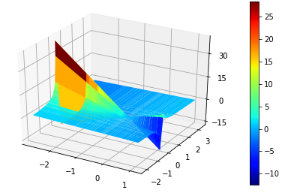
\includegraphics{figures/plot_of_division_function.png}
\caption{Topographical surface representation of the division function; $z=\frac{x}{y}$.}
\end{center}
\label{fig:div_fx}
\end{figure}

\begin{figure}
\begin{center}
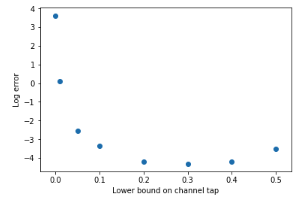
\includegraphics{figures/One_tap_channel_inversion.png}
\caption{One tap channel inversion with respect to range.}
\end{center}
\label{fig:one_tap_inv}
\end{figure}

\subsection{Learning to multiply two inputs}
NN given x, y - output x*y

\begin{figure}
\begin{center}
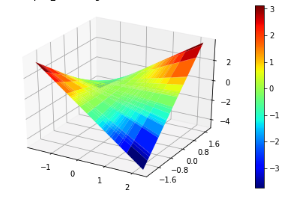
\includegraphics{figures/plot_of_multiplication_func.png}
\caption{Topographical surface representation of the multiplication function; $z=xy$.}
\end{center}
\label{fig:mult_fx}
\end{figure}

\begin{figure}
\begin{center}
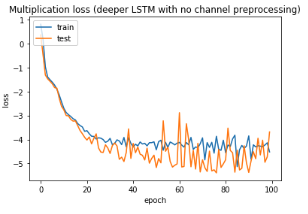
\includegraphics{figures/LSTM_loss_multiplication.png}
\caption{LSTM loss trying to learn the Multiplication function; $z=xy$.}
\end{center}
\label{fig:lstm_loss_mult}
\end{figure}


\section{Channel Equalization}

\begin{itemize}
\item compare to MMSE
\item re run with the new RNN architecture
\item backprop length of ~ 3. crude search from 1-10. 2 tap channel
\item added channel preprocessing: didn't seem to make too much of a difference
\item plot log/ log scale to find converging in error
\end{itemize}

\begin{figure}
\begin{center}
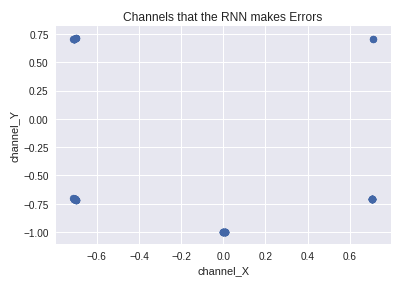
\includegraphics{figures/incorrect_channels.png}
\caption{What two tap channels does the equalizer get wrong?}
\end{center}
\label{fig:incorr_chan}
\end{figure}

\section{Channel Est + Equal}
re run that 